\input ../SlidePreamble
\input ../preamble


\begin{document}

{\Huge
  \centerline{\bf TTIC 31230,  Fundamentals of Deep Learning}
  \vfill
  \centerline{David McAllester, Autumn   2023}
  \vfill
  \centerline{\bf Contrastive Coding}
  \vfill
  \vfill

\slide{Review: Cross Entropy Loss}

$${\color{red} \argmin_\Phi E_{(x,y)\sim \pop}\left[-\ln P_\Phi(y|x)\right]}$$

\vfill
Under universality:

$${\color{red} P_{\Phi^*}(y|x) = P_{\pop}(y|x)}$$

\slide{Review: GANs}

Generative Adversarial Networks
Ian J. Goodfellow et al, 2014

\vfill
$${\color{red} \argmax_{\gen} \min_{\disc} E_{i \sim \{-1,1\}, y \sim P_i}\left[-\ln P_{\disc}(i|y)\right]}$$

\vfill
Under Universality:

\vfill
$${\color{red} P_\gen(y) = P_{\pop}(y)}$$

\slide{Review: VAEs}

Auto-Encoding Variational Bayes, Kingma and Welling, 2013

\vfill
$${\color{red} \argmin_{\pri,\dec,\enc}\;E_{y \sim \pop,z \sim P_\enc(z|y)}\left[ - \ln \frac{P_\pri(z)P_\dec(y|z)}{P_\enc(z|y)}\right]}$$

\vfill
Under Universality:

\vfill
For for any encoder $\enc$

\vfill
$${\color{red} P_{\pri^*,\dec^*}(z,y) = P_{\pop,\enc}(z,y)}$$

\vfill
Under universality the Encoder can be anything (but in practice the encoder matters).

\slide{Contrastive Coding: A Fourth Training Objective}

Representation Learning with Contrastive Predictive Coding,
Aaron van den Oord, Yazhe Li, Oriol Vinyals, July 2018.

\vfill
CLIP: Contrastive Language-Image Pre-training, January 2021, OpenAI



\slide{CLIP Contrastive Coding}

\centerline{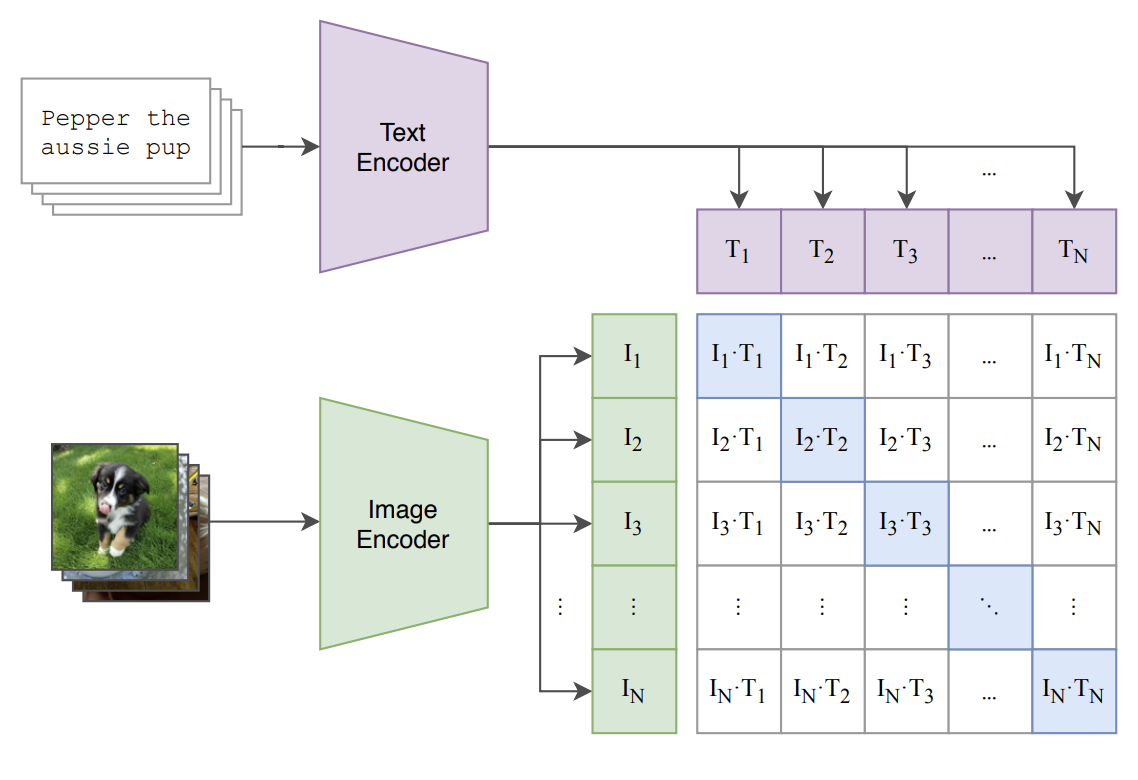
\includegraphics[height= 5in]{\images/CLIPTraining}}

\slide{Contrastive Coding: the Fourth Training Objective}

We draw pairs $(x_1,y_1), \ldots (x_B,y_B)$ from the population.
We then select $b$ uniformly from $1$ to $B$ and construct the tuple $(x_b,y_1,\ldots,y_B,b)$.

\vfill
We then train a model to predict $b$.
\vfill
{\huge
\begin{eqnarray*}
\enc_x^*,\enc_y^* & = & \argmin_{\enc_x,\enc_y} \;E_{(x_b,y_1,\ldots,y_B,b)}\left[-\ln P_{\enc_x,\enc_y}(b|x_b,y_1,\ldots,y_B)\right]
\end{eqnarray*}

\begin{eqnarray*}
P_{\enc_x,\enc_y}(b|x,y_1,\ldots,y_B) & = & \softmax_b\; \enc_x(x)^\top\enc_y(y_b)
\end{eqnarray*}
}

\slide{CLIP Contrastive Coding}

In CLIP we make $B^2$ predictions for a batch of size $N = B$
\centerline{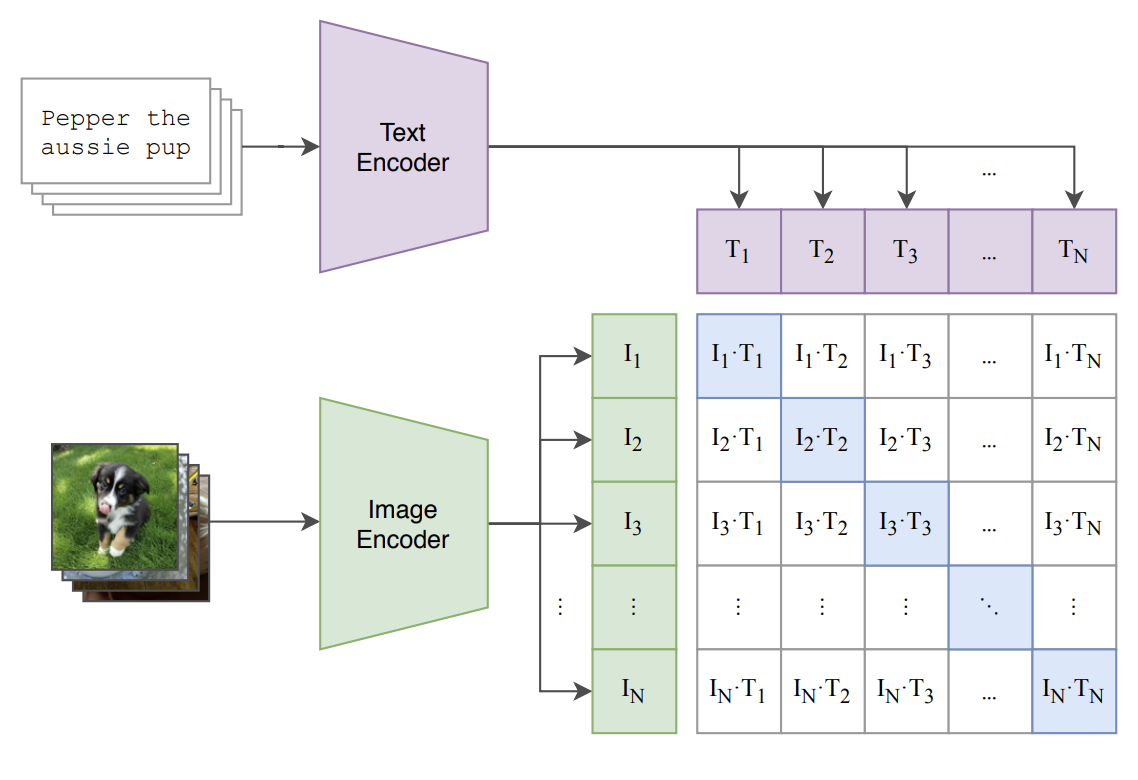
\includegraphics[height= 4in]{\images/CLIPTraining}}


\slide{The Mutual Information Contrastive Coding Theorem}

For any distribution on pairs $(x,y)$, with contrastive probabilities computed by

\begin{eqnarray*}
P(b|x,y_1,\ldots,y_B) & = & \softmax_b\;\enc_x(x),\enc_y(y_b)
\end{eqnarray*}

{\huge
\begin{eqnarray*}
I(x,y) & \geq & \ln B - \;\;E_{(x_b,y_1,\ldots,y_B,b)}\left[-\ln P(b|(x_b,y_1,\ldots,y_B))\right]
\end{eqnarray*}
}

Chen et al., On Variational Bounds of Mutual Information, May 2019.

\slide{CLIP Image Classification}

\centerline{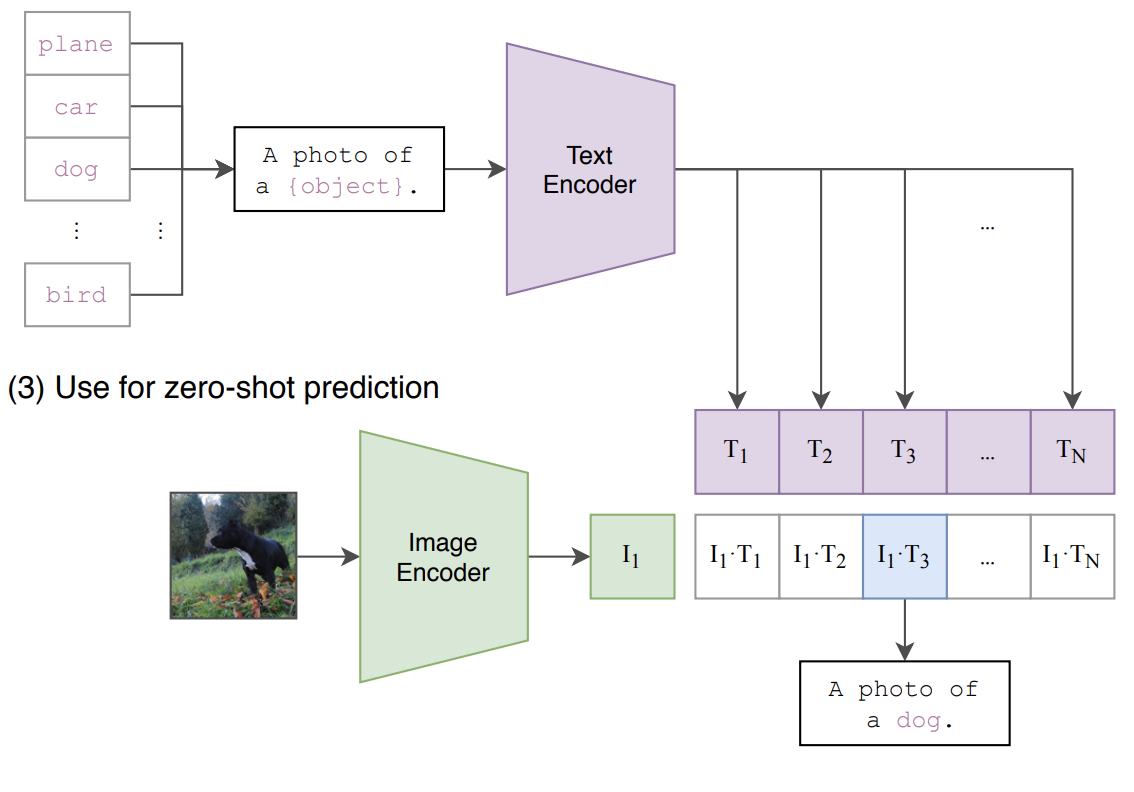
\includegraphics[height= 5in]{\images/CLIPClassifier}}

\slide{Zero-Shot Image Classification}

\centerline{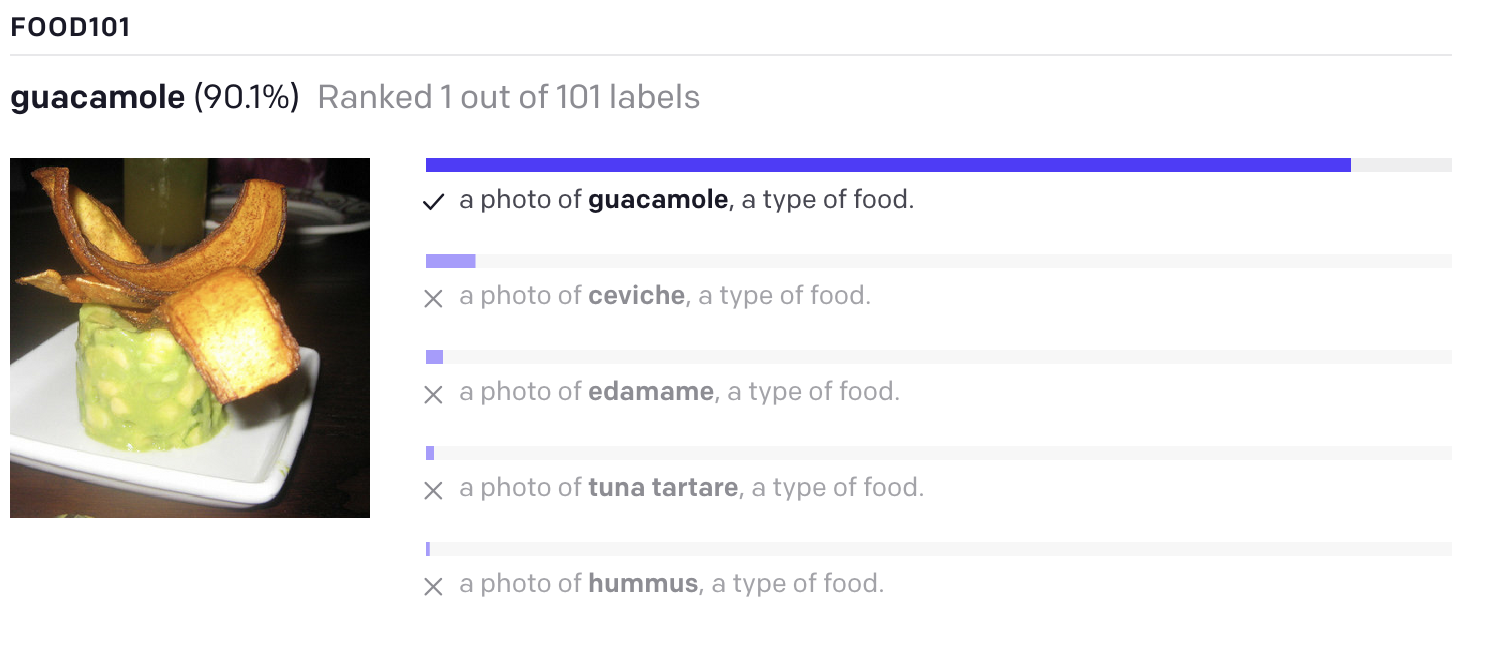
\includegraphics[width = 7in]{\images/CLIP0}}

\slide{Zero-Shot Image Classification}

\centerline{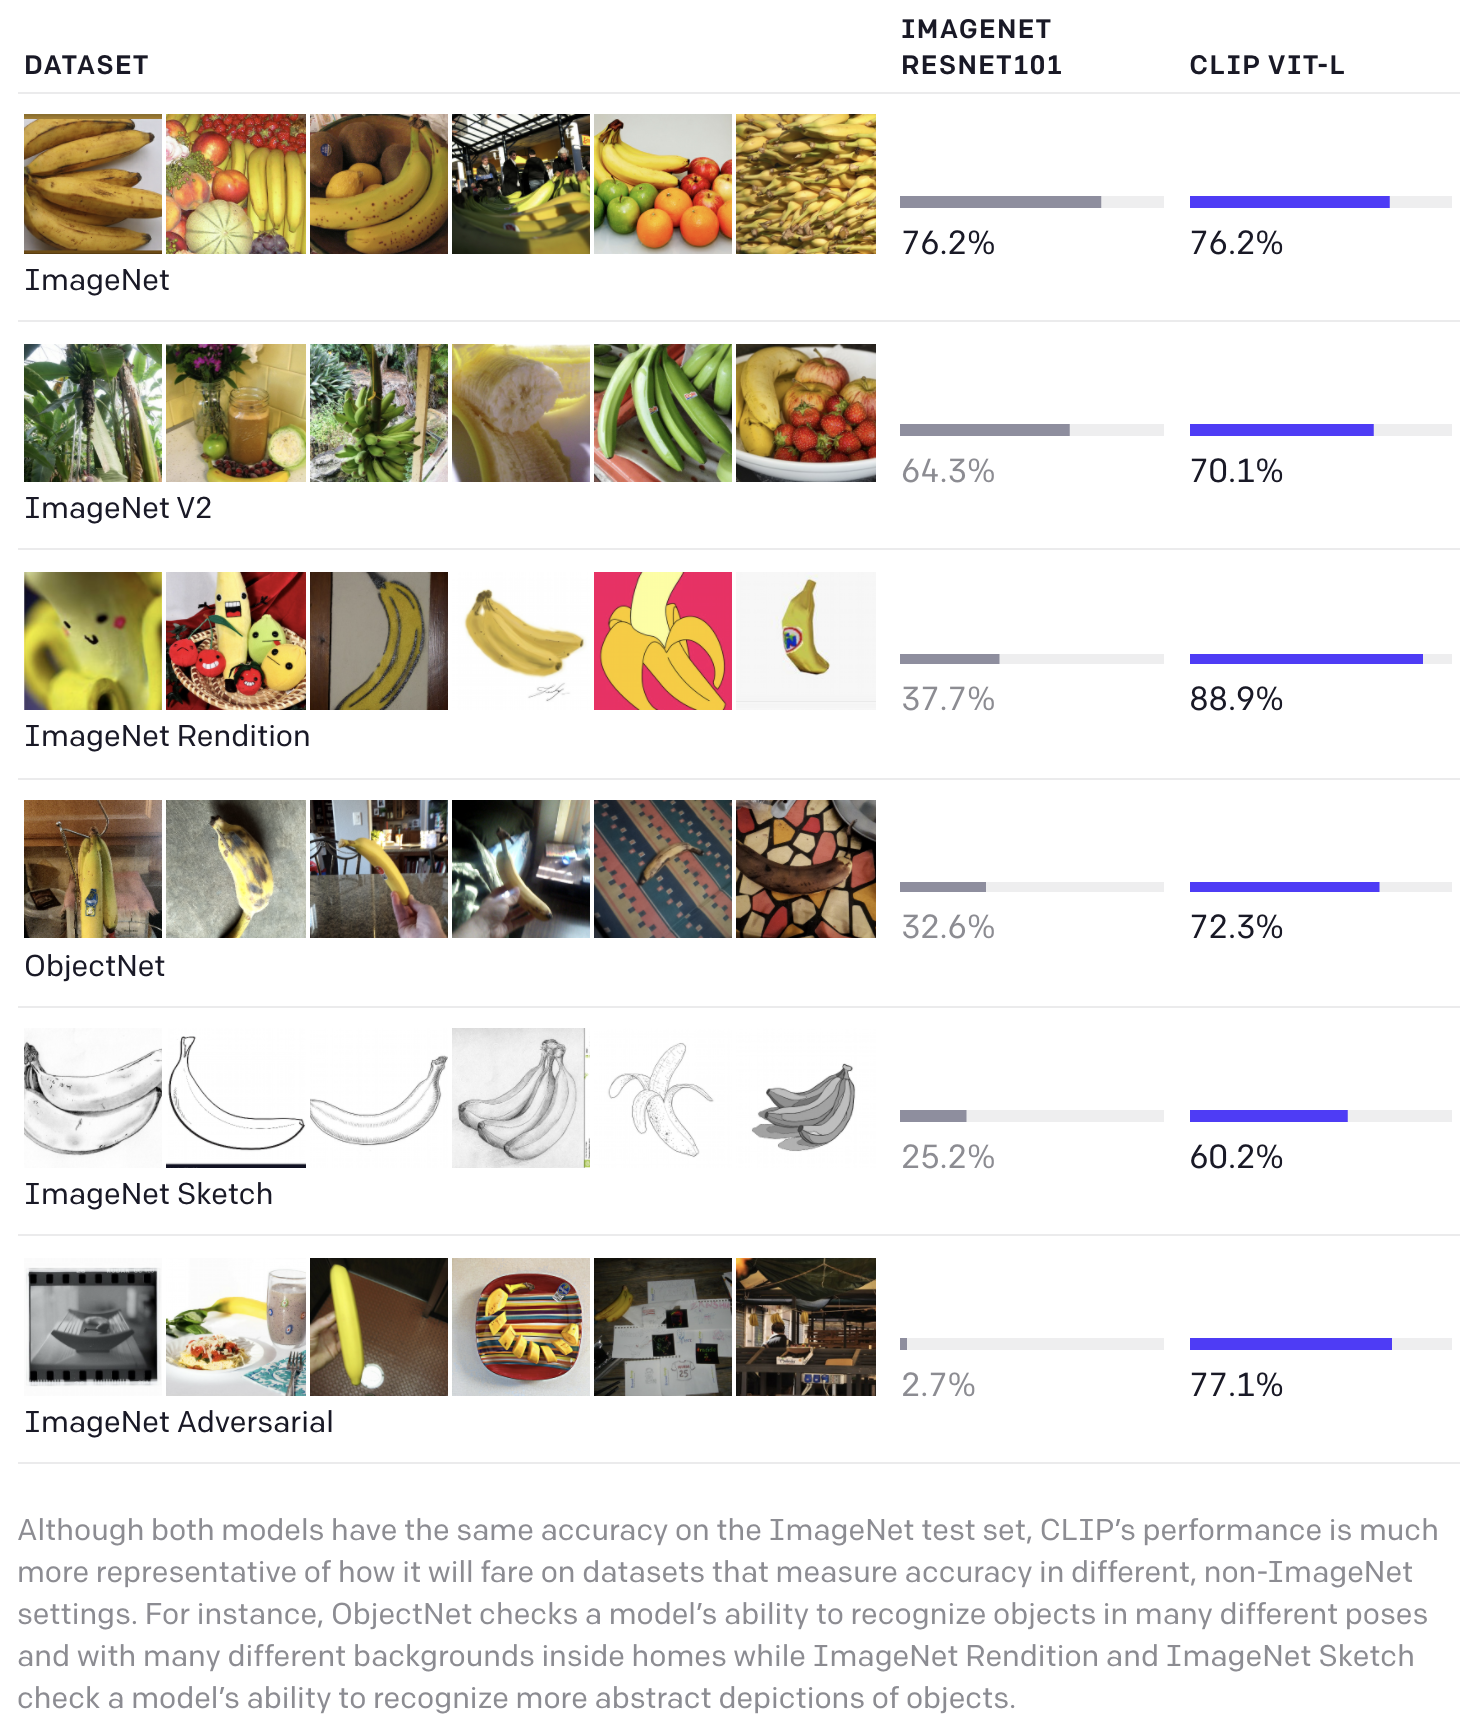
\includegraphics[height= 5in]{\images/CLIP1}}

\slide{An abstract Formulation}

 We consider a population distribution on pairs $(x,y)$.
 
 \vfill
 For example:
 
 \vfill
\begin{itemize}
\item $x$ might be an image and $y$ might be the text of a caption for image $x$ (CLIP).

\vfill
\item $x$ might be an video frame and $y$ video frame a second later.

\vfill
\item $x$ might be a window of a sound wave and $y$ a later window (Wav2Vec).

\vfill
\item $x = f(z)$ and $y = f(z)$ where $f$ and $g$ are transformation functions on an image $z$ such as  translation, rotation, color shift, or cropping. (augmentation) of $x$. (SimCLR)
\end{itemize}


\slide{A Weakness of Contrastive Coding}

{\huge
\begin{eqnarray*}
I(x,y) & \geq & \ln B - \;\;E_{(x,y_1,\ldots,y_B,b)}\left[-\ln P(b|(x,y_1,\ldots,y_B)\right]
\end{eqnarray*}
}

The discrimination problem may be too easy.

\vfill
The guarantee can never be stronger than $\ln B$ where $B$ is the batch size.

\vfill
Suppose we have 100 bits of mutual information as seem plausible for translation pairs.

\slide{Addresses the Weakness with Large Batch Size}

\begin{eqnarray*}
I(x,y) & \geq & \ln B - \;\;E_{(x,y_1,\ldots,y_B,b)}\left[-\ln P(b|(x,y_1,\ldots,y_B)\right]
\end{eqnarray*}

\vfill
For CLIP the batch size $B = 2^{15}$ so we can potentially guarantee 15 bits of mutual information.


\slide{Contrastive Coding for Speech}
\centerline{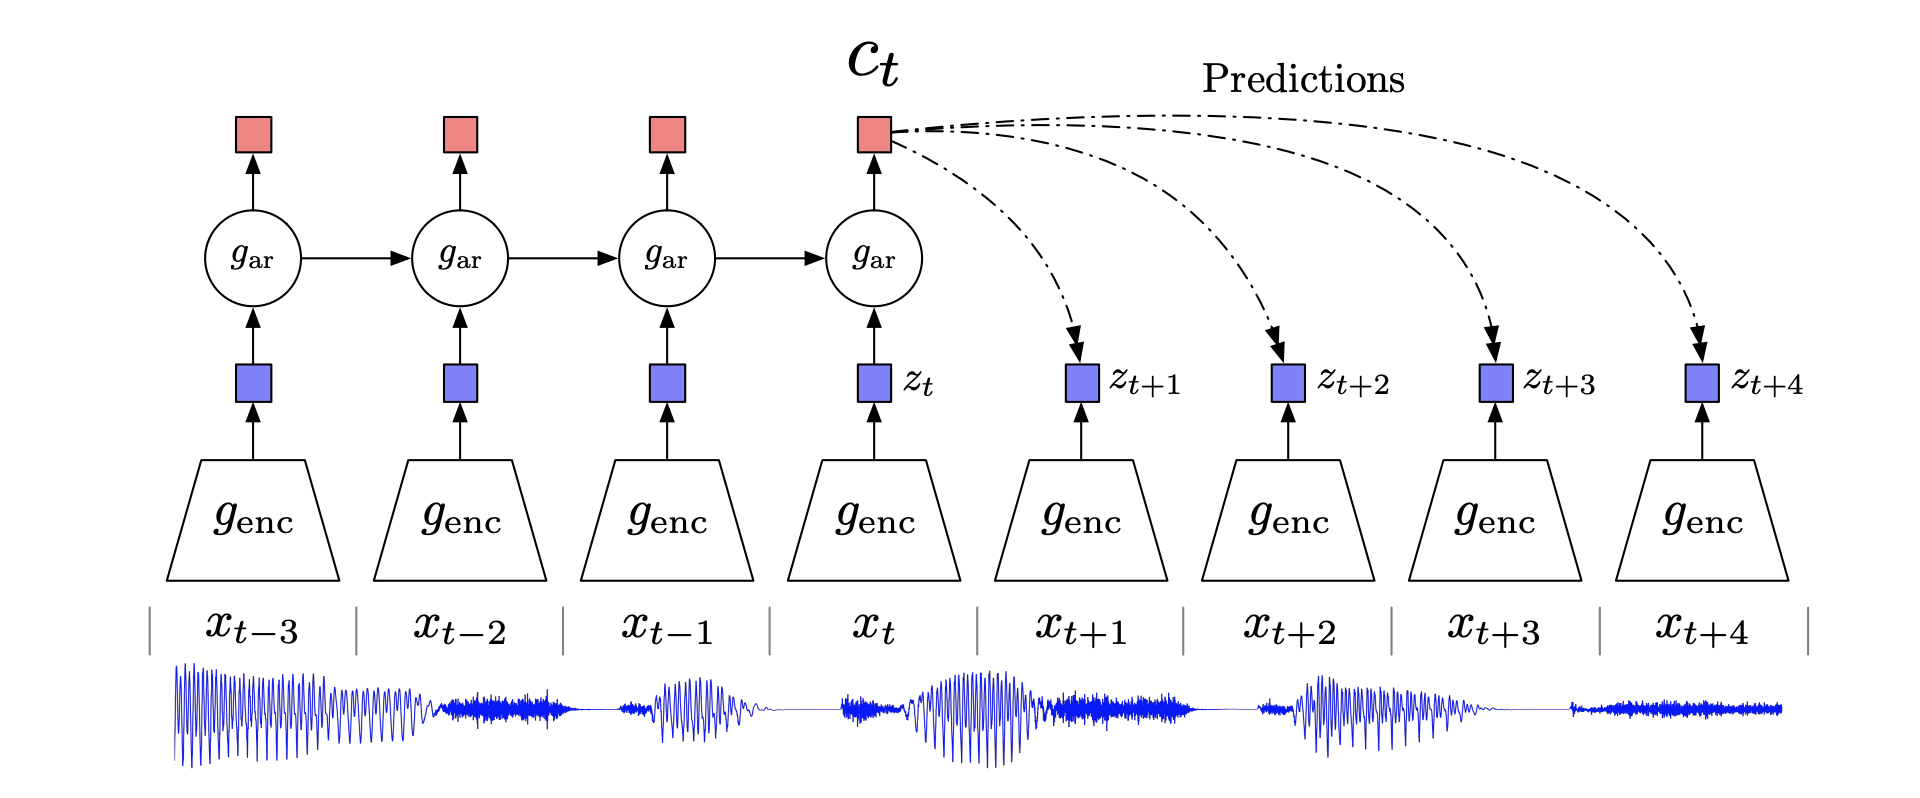
\includegraphics[width = 6 in]{\images/CPC}}
\centerline{\huge van den Oord, Li and Vinyals,}
\centerline{\huge Representation Learning with Contrastive Predictive Coding, 2018}

\vfill
What should we abstract from the past that is relevant to the future?

\slide{Contrastive Coding for Speech}
\centerline{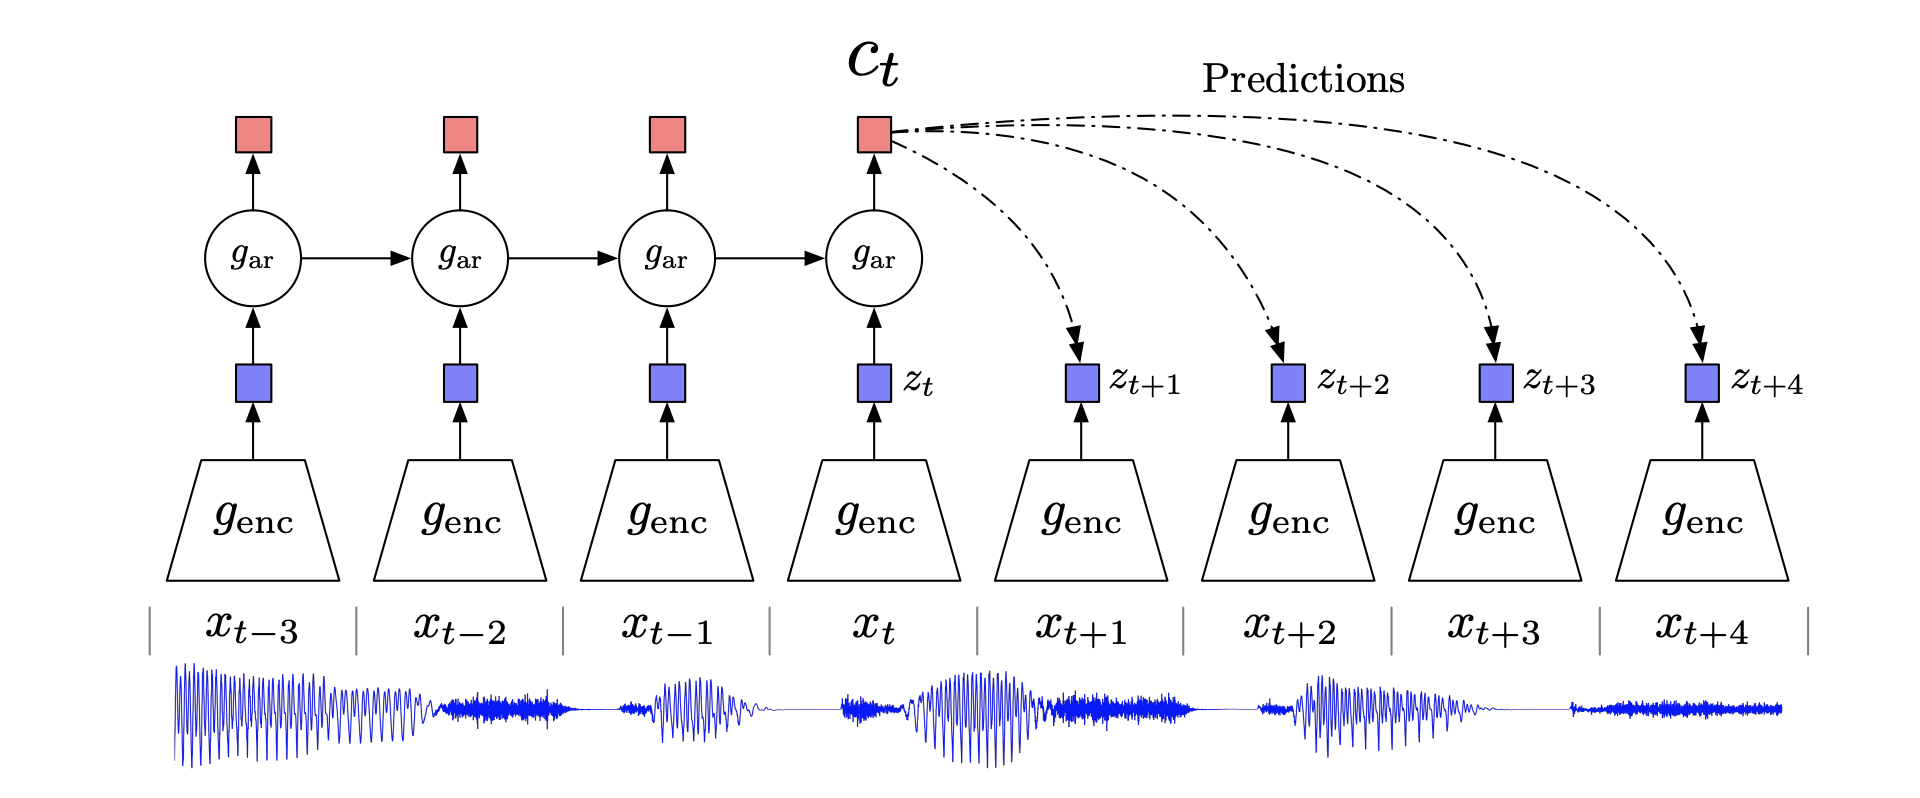
\includegraphics[width = 6 in]{\images/CPC}}

\vfill
{\bf Unlike VAEs}, contrastive coding is about {\bf capturing mutual information}.
Intuitively we want to {\bf separate signal from noise} and avoid modeling noise.

\slide{Contrastive Coding for Speech}
\centerline{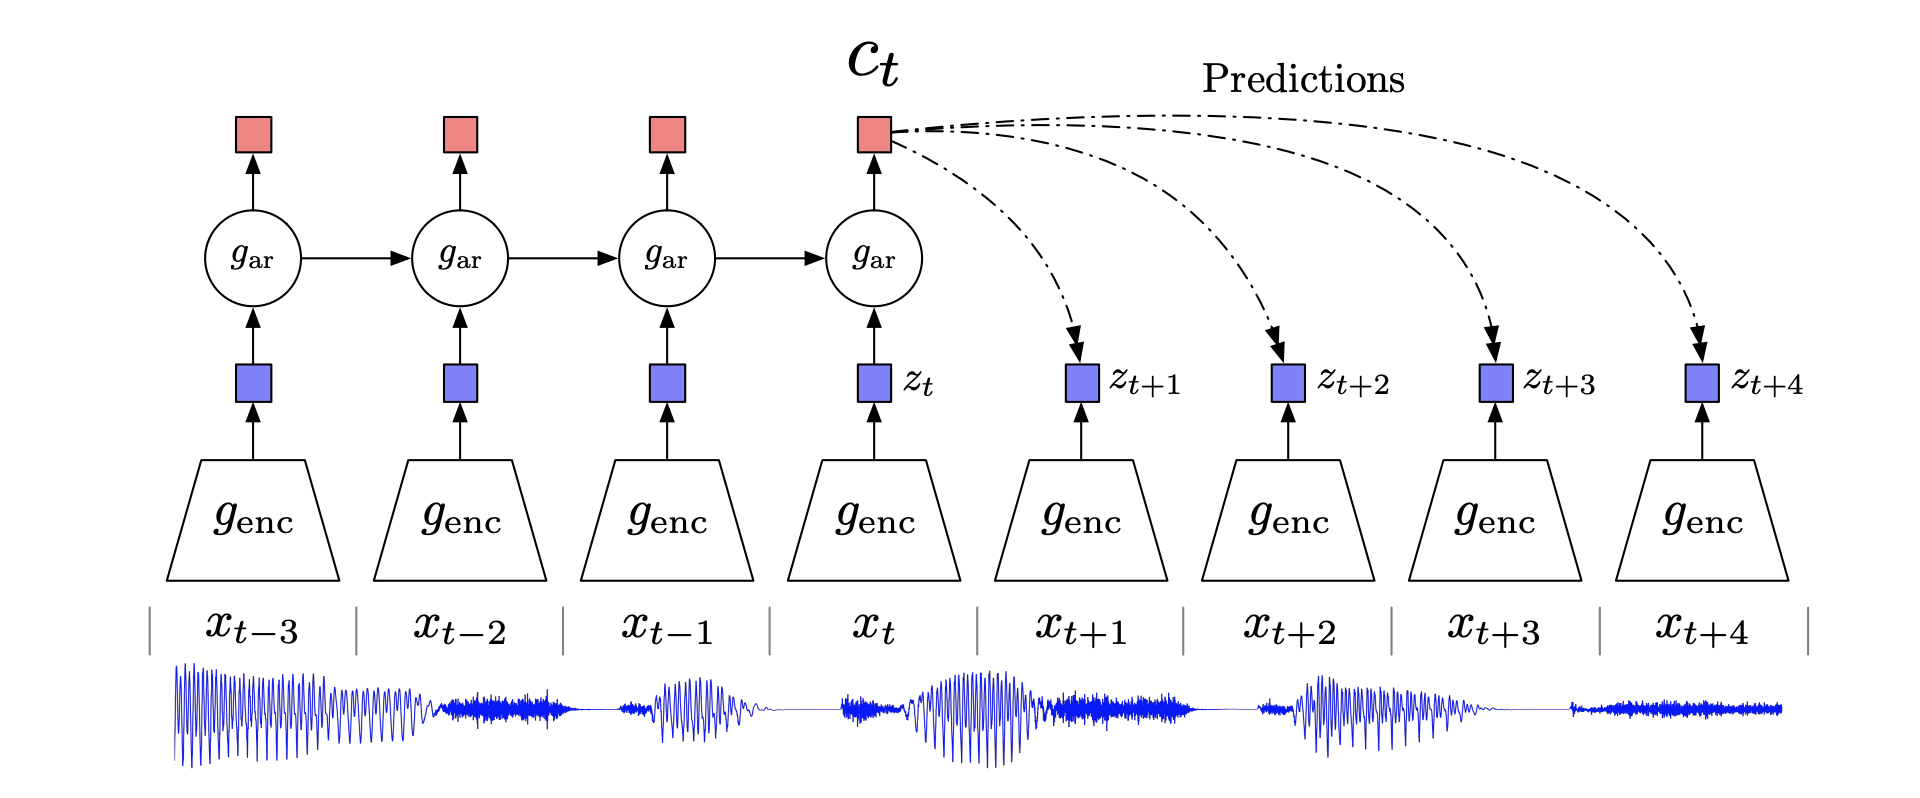
\includegraphics[width = 6 in]{\images/CPC}}

\vfill
We abstract this problem to that of capturing the mutual information between any two arbitrary random variables $x$ and $y$.

\slide{Tishby's Information Bottleneck}

\centerline{The Information Bottleneck Method}
\centerline{Tishby, Pereira and Bialeck, 1999}

\vfill
Design $P_\enc(z|x)$ with the following objective.

\vfill
$$\enc^* = \argmin_\enc\;I(z,x) - \beta I(z,y)$$

\slide{END}

}
\end{document}

